\chapter{Number Theory and Cryptography}\index{number theory}

Every time you log in to a website, your phone and a server you have never met
agree on a secret, while anyone on the network can listen in. That sounds
impossible. It works because of a few facts about whole numbers, some of them
more than 2,000 years old. Multiplying two huge primes is easy; un-multiplying
the result is so hard that no computer on Earth can do it in a lifetime. In
this chapter, you will learn the number theory behind that idea and then use
it to build \newterm{RSA}, the system that protected the internet for decades.

\section{Divisibility}\index{divisibility}

We say that $a$ \newterm{divides} $b$, written $a \mid b$, if $b = ak$ for
some integer $k$. Then $a$ is a \newterm{divisor} (or \newterm{factor}) of
$b$, and $b$ is a \newterm{multiple} of $a$. For example, $3 \mid 12$ because
$12 = 3 \cdot 4$, but $5 \nmid 12$. Do not confuse $a \mid b$, which is a
statement (true or false), with $a / b$, which is a number.

Divisibility facts are perfect practice for the direct proofs from the
Proofs chapter.

\begin{theorem}
If $a \mid b$ and $a \mid c$, then $a \mid (b + c)$.
\end{theorem}
\begin{proof}
Since $a \mid b$ and $a \mid c$, there are integers $j$ and $k$ with $b = aj$
and $c = ak$. Then $b + c = aj + ak = a(j + k)$. Because $j + k$ is an
integer, $a \mid (b + c)$.
\end{proof}

\subsection{The Division Algorithm}\index{division algorithm}
When $b$ does not divide $a$ evenly, there is a remainder. For any integer
$a$ and any positive integer $b$, there is exactly one way to write
$$a = qb + r \qquad \text{with } 0 \leq r < b$$
The number $q$ is the \newterm{quotient} and $r$ is the
\newterm{remainder}. In Python, \mintinline{python}{a // b} gives $q$ and
\mintinline{python}{a % b} gives $r$. For example, $100 = 14 \cdot 7 + 2$,
and \mintinline{python}{100 // 7} is $14$ while \mintinline{python}{100 % 7}
is $2$.

The remainder is never negative, even when $a$ is: $-17 = (-4)\cdot 5 + 3$,
so the remainder is $3$, not $-2$. Python agrees:
\mintinline{python}{-17 % 5} is $3$.

\begin{Exercise}[title={Quotients and Remainders}, label=nt_div]
Write each in the form $a = qb + r$ with $0 \leq r < b$.
\begin{enumerate}
\item $a = 100$, $b = 7$
\item $a = 2026$, $b = 12$
\item $a = -17$, $b = 5$
\end{enumerate}
\end{Exercise}
\begin{Answer}[ref=nt_div]
\begin{enumerate}
\item $100 = 14 \cdot 7 + 2$
\item $2026 = 168 \cdot 12 + 10$
\item $-17 = (-4) \cdot 5 + 3$
\end{enumerate}
\end{Answer}

\begin{Exercise}[title={A Divisibility Proof}, label=nt_trans]
Prove that if $a \mid b$ and $b \mid c$, then $a \mid c$.
\end{Exercise}
\begin{Answer}[ref=nt_trans]
Since $a \mid b$, there is an integer $j$ with $b = aj$. Since $b \mid c$, there
is an integer $k$ with $c = bk$. Substituting, $c = (aj)k = a(jk)$. Because $jk$
is an integer, $a \mid c$.
\end{Answer}

\section{Prime Numbers}\index{prime number}

A \newterm{prime} is an integer greater than 1 whose only positive divisors
are 1 and itself. The first few are
$$2, 3, 5, 7, 11, 13, 17, 19, 23, 29, \dots$$
An integer greater than 1 that is not prime is \newterm{composite}. The
number 1 is neither prime nor composite. (Leaving it out makes the next
theorem work.)

\begin{theorem}[Fundamental Theorem of Arithmetic]\index{Fundamental Theorem of Arithmetic}
Every integer greater than 1 can be written as a product of primes in exactly
one way, apart from the order of the factors.
\end{theorem}

For example, $360 = 2^3 \cdot 3^2 \cdot 5$. You can find a factorization by
splitting off one factor at a time ($360 = 2 \cdot 180 = 2 \cdot 2 \cdot 90 =
\cdots$), and no matter which factors you split off first, you end up with the
same primes. Primes are the atoms of multiplication: every whole number is
built from them in exactly one way.

\subsection{There Are Infinitely Many Primes}
Primes get rarer as numbers get bigger. Do they ever run out? Euclid answered
this around 300 BCE with one of the most famous proofs by contradiction ever
written.

\begin{theorem}
There are infinitely many primes.
\end{theorem}
\begin{proof}
Suppose, for contradiction, that there are only finitely many primes,
$p_1, p_2, \dots, p_k$. Let
$$N = p_1 p_2 \cdots p_k + 1$$
$N$ is greater than 1, so it has at least one prime factor $p$. That prime
must be one of $p_1, \dots, p_k$, so $p$ divides the product
$p_1 p_2 \cdots p_k$. Since $p$ also divides $N$, it divides the difference
$N - p_1 p_2 \cdots p_k = 1$. But no prime divides 1. This contradiction
shows that our list could not have contained every prime.
\end{proof}

\subsection{Testing Whether a Number Is Prime}\index{trial division}
To check whether $n$ is prime, you could try dividing it by every number from
2 to $n - 1$. You can stop much sooner. If $n = ab$ with $1 < a \leq b$, then
$a \cdot a \leq a \cdot b = n$, so $a \leq \sqrt{n}$. In other words, a
composite number always has a factor no bigger than its square root. So you only
need to try primes up to $\sqrt{n}$. This is called \newterm{trial division}.

\textbf{Example}: Is 221 prime?

\textbf{Solution}: $\sqrt{221} \approx 14.9$, so we try the primes 2, 3, 5, 7,
11, and 13. The first five leave remainders, but $221 = 13 \cdot 17$. It is
composite.

\subsection{The Sieve of Eratosthenes}\index{Sieve of Eratosthenes}
To find \emph{all} the primes up to some limit, the Greek astronomer
Eratosthenes had a cleverer idea. Write down the numbers from 2 to the limit.
Circle 2 and cross out every multiple of 2. The next number not crossed out, 3,
is prime: circle it and cross out its multiples. Repeat. Every number still
standing at the end is prime. You can stop once you reach the square root of
the limit, for the same reason as in trial division.

\begin{minted}{python}
def primes_up_to(n):
    is_prime = [True] * (n + 1)
    is_prime[0] = is_prime[1] = False
    for p in range(2, int(n ** 0.5) + 1):
        if is_prime[p]:
            # cross out every multiple of p, starting at p * p
            for multiple in range(p * p, n + 1, p):
                is_prime[multiple] = False
    return [k for k in range(n + 1) if is_prime[k]]

print(primes_up_to(50))
print(len(primes_up_to(1_000_000)))
\end{minted}
\begin{verbatim}
[2, 3, 5, 7, 11, 13, 17, 19, 23, 29, 31, 37, 41, 43, 47]
78498
\end{verbatim}
There are 78,498 primes below one million, and the sieve finds them all in
about a second.

\begin{Exercise}[title={Factor and Test}, label=nt_primes]
\begin{enumerate}
\item Find the prime factorization of $1001$.
\item Is $391$ prime? Which primes do you need to try?
\end{enumerate}
\end{Exercise}
\begin{Answer}[ref=nt_primes]
\begin{enumerate}
\item $1001 = 7 \cdot 11 \cdot 13$.
\item $\sqrt{391} \approx 19.8$, so try 2, 3, 5, 7, 11, 13, 17, and 19. It is
not divisible by 2 through 13, but $391 = 17 \cdot 23$. It is composite.
\end{enumerate}
\end{Answer}

\section{The Greatest Common Divisor}\index{greatest common divisor}

The \newterm{greatest common divisor} of two integers, $\gcd(a, b)$, is the
largest integer that divides both. For example, $\gcd(12, 18) = 6$. If
$\gcd(a, b) = 1$, we say $a$ and $b$ are \newterm{relatively prime}: they
share no prime factor.

You could find a gcd by factoring both numbers, but factoring big numbers is
hard. (That is the whole point of RSA!) Fortunately, there is a much faster way.

\subsection{The Euclidean Algorithm}\index{Euclidean algorithm}
The key fact is this: if $a = qb + r$, then
$$\gcd(a, b) = \gcd(b, r)$$
Why? Any number that divides $a$ and $b$ also divides $r = a - qb$, and any
number that divides $b$ and $r$ also divides $a = qb + r$. So the two pairs
have exactly the same common divisors, and therefore the same greatest one.

So replace $(a, b)$ by $(b, r)$ and repeat. The numbers shrink every step, and
when the remainder reaches 0, the last nonzero remainder is the gcd.

\textbf{Example}: Find $\gcd(1071, 462)$.

\textbf{Solution}:
\begin{align*}
1071 &= 2 \cdot 462 + 147 \\
462 &= 3 \cdot 147 + 21 \\
147 &= 7 \cdot 21 + 0
\end{align*}
The last nonzero remainder is 21, so $\gcd(1071, 462) = 21$. Three divisions,
no factoring.

In Python, the algorithm is four lines long:
\begin{minted}{python}
def gcd(a, b):
    while b != 0:
        a, b = b, a % b
    return a

print(gcd(1071, 462))
print(gcd(252, 198))
\end{minted}
\begin{verbatim}
21
18
\end{verbatim}
(Python's \mintinline{python}{math} library also has a built-in
\mintinline{python}{math.gcd}.) The Euclidean algorithm is fast even for
numbers with hundreds of digits, because the remainders shrink by at least
half every two steps.

\subsection{The Extended Euclidean Algorithm}\index{Bezout's identity@B\'ezout's identity}
Running the algorithm backward reveals something surprising: the gcd can
always be written as a combination of the two numbers. For any integers $a$
and $b$, there are integers $x$ and $y$ with
$$ax + by = \gcd(a, b)$$
This is called \newterm{B\'ezout's identity}. To find $x$ and $y$, solve each
step of the algorithm for its remainder, then substitute upward. For
$1071$ and $462$:
\begin{align*}
21 &= 462 - 3 \cdot 147 \\
   &= 462 - 3 \cdot (1071 - 2 \cdot 462) \\
   &= 7 \cdot 462 - 3 \cdot 1071
\end{align*}
So $x = -3$ and $y = 7$: indeed, $1071(-3) + 462(7) = -3213 + 3234 = 21$.
This back-substitution is exactly what RSA needs to build its secret key.

\begin{Exercise}[title={Euclid by Hand}, label=nt_gcd]
\begin{enumerate}
\item Use the Euclidean algorithm to find $\gcd(252, 198)$.
\item Find integers $x$ and $y$ with $252x + 198y = \gcd(252, 198)$.
\end{enumerate}
\end{Exercise}
\begin{Answer}[ref=nt_gcd]
\begin{enumerate}
\item
\begin{align*}
252 &= 1 \cdot 198 + 54 \\
198 &= 3 \cdot 54 + 36 \\
54 &= 1 \cdot 36 + 18 \\
36 &= 2 \cdot 18 + 0
\end{align*}
So $\gcd(252, 198) = 18$.
\item Work backward:
\begin{align*}
18 &= 54 - 36 = 54 - (198 - 3 \cdot 54) = 4 \cdot 54 - 198 \\
   &= 4(252 - 198) - 198 = 4 \cdot 252 - 5 \cdot 198
\end{align*}
So $x = 4$ and $y = -5$. Check: $1008 - 990 = 18$.
\end{enumerate}
\end{Answer}

\section{Modular Arithmetic}\index{modular arithmetic}

If it is 9 o'clock now, what time will it be in 5 hours? Not 14 o'clock: the
clock wraps around, and it will be 2 o'clock. You already do
\newterm{modular arithmetic}: arithmetic where numbers wrap around after
reaching a fixed value, called the \newterm{modulus}.

\begin{figure}[H]
\centering
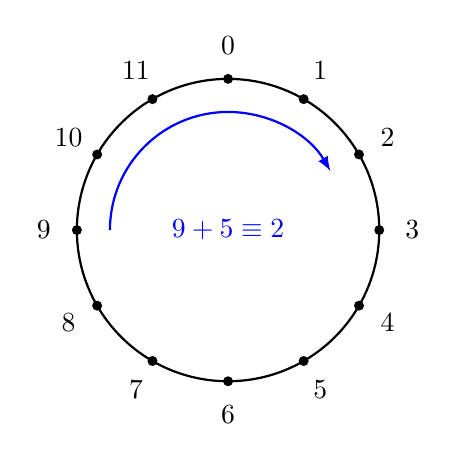
\begin{tikzpicture}[scale=1.2]
\draw[thick] (0,0) circle (1.6);
\foreach \k in {0,...,11} {
  \pgfmathsetmacro{\ang}{90 - 30*\k}
  \fill (\ang:1.6) circle (1.5pt);
  \node at (\ang:1.95) {\k};
}
\draw[-latex, thick, blue] (90-30*9:1.25) arc (90-30*9:90-30*14:1.25);
\node[blue] at (0,0) {$9 + 5 \equiv 2$};
\end{tikzpicture}
\caption{Arithmetic mod 12. Starting at 9 and moving 5 steps lands on 2.}
\label{fig:clock-mod12}
\end{figure}

\begin{definition}
Let $n$ be a positive integer. We say $a$ is \newterm{congruent} to $b$ modulo
$n$, written
$$a \equiv b \pmod{n}$$
if $n \mid (a - b)$. Equivalently, $a$ and $b$ leave the same remainder when
divided by $n$.
\end{definition}

For example, $14 \equiv 2 \pmod{12}$, $17 \equiv 2 \pmod{5}$, and
$-1 \equiv 11 \pmod{12}$ (one hour before midnight is 11 o'clock).

The great thing about congruences is that you can reduce at any time. If
$a \equiv b$ and $c \equiv d \pmod{n}$, then
$$a + c \equiv b + d \pmod{n} \qquad \text{and} \qquad ac \equiv bd \pmod{n}$$
So you can replace any number by its remainder before adding or multiplying.
That keeps the numbers small, even when the true answer is enormous.

\textbf{Example}: What is the last digit of $3^{2026}$?

\textbf{Solution}: The last digit of a number is its remainder mod 10. The
powers of 3 mod 10 are
$$3^1 \equiv 3, \quad 3^2 \equiv 9, \quad 3^3 \equiv 27 \equiv 7, \quad 3^4 \equiv 21 \equiv 1$$
Once we hit 1, the pattern repeats every 4 steps. Since $2026 = 4 \cdot 506 + 2$,
$$3^{2026} = \left(3^4\right)^{506} \cdot 3^2 \equiv 1^{506} \cdot 9 = 9 \pmod{10}$$
The last digit is 9, even though $3^{2026}$ has 967 digits.

\subsection{Modular Inverses}\index{modular inverse}
In ordinary arithmetic, dividing by 3 means multiplying by $\frac{1}{3}$, the
number whose product with 3 is 1. Mod $n$, there are no fractions, but there can
still be a number that acts like $\frac{1}{3}$. An \newterm{inverse} of $a$
modulo $n$ is a number $x$ with
$$ax \equiv 1 \pmod{n}$$
For example, $3 \cdot 4 = 12 \equiv 1 \pmod{11}$, so 4 is the inverse of 3 mod
11.

Not every number has an inverse. Mod 12, no multiple of 4 is ever 1 more than a
multiple of 12. (Multiples of 4 are always multiples of 4, and $12k + 1$ never
is.) In general, $a$ has an inverse mod $n$ exactly when $\gcd(a, n) = 1$, and
the extended Euclidean algorithm finds it: if $ax + ny = 1$, then
$ax \equiv 1 \pmod{n}$. In Python, \mintinline{python}{pow(a, -1, n)} computes
it for you.

\subsection{Fast Powers}\index{modular exponentiation}
RSA needs numbers like $m^{e} \bmod n$, where all three numbers have hundreds of
digits. Multiplying $m$ by itself $e$ times would take longer than the age of
the universe. Instead, use \newterm{repeated squaring}: square, reduce,
square, reduce. To compute $5^{13} \bmod 23$, write $13 = 8 + 4 + 1$ and find
\begin{align*}
5^1 &\equiv 5 \\
5^2 &\equiv 25 \equiv 2 \\
5^4 &\equiv 2^2 = 4 \\
5^8 &\equiv 4^2 = 16
\end{align*}
Then $5^{13} = 5^8 \cdot 5^4 \cdot 5^1 \equiv 16 \cdot 4 \cdot 5 = 320 \equiv 21
\pmod{23}$. That is five multiplications instead of twelve. For an exponent with
600 digits, it is a few thousand multiplications instead of a number with 600
digits. Python's three-argument \mintinline{python}{pow(m, e, n)} uses this
method.

\begin{Exercise}[title={Wrapping Around}, label=nt_mod]
\begin{enumerate}
\item What is the last digit of $7^{2026}$?
\item Find the inverse of 5 modulo 12. Check your answer.
\item Explain why 6 has no inverse modulo 9.
\end{enumerate}
\end{Exercise}
\begin{Answer}[ref=nt_mod]
\begin{enumerate}
\item The powers of 7 mod 10 are 7, 9, 3, 1, then repeat every 4. Since
$2026 = 4 \cdot 506 + 2$, $7^{2026} \equiv 7^2 \equiv 9$. The last digit is 9.
\item $5 \cdot 5 = 25 = 2 \cdot 12 + 1 \equiv 1 \pmod{12}$, so 5 is its own inverse.
\item $\gcd(6, 9) = 3$, not 1. Every multiple of 6 is a multiple of 3, and so is
every number of the form $9k$, so $6x - 9k$ is always a multiple of 3 and can never
equal 1.
\end{enumerate}
\end{Answer}

\section{Fermat's Little Theorem}\index{Fermat's Little Theorem}

Try raising numbers to the 6th power mod 7:
$$1^6 \equiv 1, \quad 2^6 = 64 \equiv 1, \quad 3^6 = 729 \equiv 1, \quad \dots, \quad 6^6 = 46656 \equiv 1 \pmod{7}$$
Every one is 1. That is no accident.

\begin{theorem}[Fermat's Little Theorem]
If $p$ is prime and $p \nmid a$, then
$$a^{p-1} \equiv 1 \pmod{p}$$
\end{theorem}

\begin{proof}
Look at the $p - 1$ numbers $a, 2a, 3a, \dots, (p-1)a$, reduced mod $p$. None
of them is 0, because $p$ divides neither $a$ nor any of $1, \dots, p-1$ (and a
prime that divides a product must divide one of its factors). No two are equal
either: if $ia \equiv ja$, then $p \mid (i - j)a$, so $p \mid (i - j)$, which is
impossible for two different numbers between 1 and $p - 1$. So these are $p - 1$
different nonzero remainders, which means they are $1, 2, \dots, p-1$ in some
order. (For $p = 7$ and $a = 3$, they are $3, 6, 2, 5, 1, 4$.)

Multiply all of them together. The two lists have the same product mod $p$:
$$a \cdot 2a \cdot 3a \cdots (p-1)a \equiv 1 \cdot 2 \cdot 3 \cdots (p-1) \pmod{p}$$
$$a^{p-1} \cdot (p-1)! \equiv (p-1)! \pmod{p}$$
Since $p$ does not divide $(p-1)!$, it has an inverse mod $p$. Multiplying both
sides by that inverse leaves $a^{p-1} \equiv 1 \pmod{p}$.
\end{proof}

Fermat's Little Theorem makes huge powers easy. To find $2^{100} \bmod 13$, note
that $2^{12} \equiv 1$ and $100 = 8 \cdot 12 + 4$, so
$$2^{100} = \left(2^{12}\right)^8 \cdot 2^4 \equiv 1^8 \cdot 16 \equiv 3 \pmod{13}$$

\subsection{A Fast Primality Test}\index{Fermat primality test}
The theorem also gives a quick way to catch composite numbers. If
$a^{n-1} \not\equiv 1 \pmod{n}$, then $n$ is definitely not prime. Computers
use this, with fast powers, to test numbers with hundreds of digits in a
fraction of a second, far faster than trial division.

Passing the test does not prove $n$ is prime, though. For example,
$2^{340} \equiv 1 \pmod{341}$, but $341 = 11 \cdot 31$. A composite number that
passes is called a \newterm{pseudoprime}. Trying a different base usually
exposes it: $3^{340} \equiv 56 \pmod{341}$. Real primality tests use refined
versions of this idea that no composite can fool.

\begin{Exercise}[title={Using Fermat}, label=nt_fermat]
\begin{enumerate}
\item Use Fermat's Little Theorem to find $3^{100} \bmod 7$.
\item The number $561 = 3 \cdot 11 \cdot 17$ satisfies $2^{560} \equiv 1 \pmod{561}$.
What does this tell you about the Fermat test?
\end{enumerate}
\end{Exercise}
\begin{Answer}[ref=nt_fermat]
\begin{enumerate}
\item $3^6 \equiv 1 \pmod 7$ and $100 = 16 \cdot 6 + 4$, so
$3^{100} \equiv 3^4 = 81 \equiv 4 \pmod 7$.
\item 561 is composite but passes the test for base 2, so passing the Fermat
test does not prove a number is prime. (561 is a \emph{Carmichael number}: it
passes for every base that shares no factor with it.)
\end{enumerate}
\end{Answer}

\section{RSA}\index{RSA}

Old ciphers had a weakness: the key that locks a message also unlocks it, so
two people had to meet in secret to share a key first. In 1977, Ron Rivest,
Adi Shamir, and Leonard Adleman published a way around this. In
\newterm{public-key cryptography}, you have two keys. Your \newterm{public key}
is like an open padlock: you hand out copies to everyone, and anyone can snap
one shut on a box. Your \newterm{private key} opens the lock, and only you
have it.

In RSA, a message is a number $m$. Encrypting and decrypting are two functions,
and, just like the inverse functions you met in the Inverses and Transformations
chapter, decrypting undoes encrypting.

\subsection{Making the Keys}
\begin{enumerate}
\item Choose two different large primes, $p$ and $q$. Keep them secret.
\item Compute $n = pq$. This is public.
\item Compute $\varphi = (p - 1)(q - 1)$. Keep it secret.
\item Choose $e$ with $\gcd(e, \varphi) = 1$. This is public. (65537 is a common choice.)
\item Compute $d$, the inverse of $e$ modulo $\varphi$, with the extended
Euclidean algorithm. This is your private key.
\end{enumerate}
The public key is the pair $(n, e)$. To \textbf{encrypt} a message $m$ (a number
less than $n$), anyone computes
$$c = m^e \bmod n$$
To \textbf{decrypt}, you compute
$$m = c^d \bmod n$$

\textbf{Example}: Choose $p = 61$ and $q = 53$. Then $n = 3233$ and
$\varphi = 60 \cdot 52 = 3120$. Take $e = 17$, which shares no factor with
3120. The extended Euclidean algorithm gives $d = 2753$; check:
$17 \cdot 2753 = 46801 = 15 \cdot 3120 + 1$. To send $m = 65$, compute
$c = 65^{17} \bmod 3233 = 2790$. Only someone who knows $d$ can turn 2790 back
into the message: $2790^{2753} \bmod 3233 = 65$.

Here is the whole thing in Python:
\begin{minted}{python}
from math import gcd

# Key generation
p, q = 61, 53
n = p * q                    # public
phi = (p - 1) * (q - 1)      # secret
e = 17                       # public
assert gcd(e, phi) == 1
d = pow(e, -1, phi)          # secret: the inverse of e mod phi
print("n =", n, " phi =", phi, " d =", d)

# Encrypt and decrypt a message
m = 65
c = pow(m, e, n)             # anyone can do this with (n, e)
print("ciphertext:", c)
print("decrypted:", pow(c, d, n))   # only the key owner knows d
\end{minted}
\begin{verbatim}
n = 3233  phi = 3120  d = 2753
ciphertext: 2790
decrypted: 65
\end{verbatim}

\subsection{Why Decryption Works}
Because $ed \equiv 1 \pmod{\varphi}$, we can write $ed = 1 + k(p-1)(q-1)$ for some
integer $k$. Decrypting gives
$$c^d \equiv (m^e)^d = m^{ed} = m \cdot \left(m^{p-1}\right)^{k(q-1)} \pmod{p}$$
If $p \nmid m$, Fermat's Little Theorem says $m^{p-1} \equiv 1 \pmod{p}$, so
$m^{ed} \equiv m \cdot 1 = m \pmod{p}$. If $p \mid m$, both sides are $0 \bmod p$,
so again $m^{ed} \equiv m$. The same argument works mod $q$. So both $p$ and $q$
divide $m^{ed} - m$, and since they are different primes, so does their product
$n$. Therefore $c^d \equiv m \pmod{n}$: decryption returns the original message.

\subsection{Why It Is Secure}
Everyone knows $n$ and $e$. To find $d$, an attacker needs $\varphi$, and to
find $\varphi$, they need $p$ and $q$. That means factoring $n$. For our toy
key, $n = 3233$ falls to trial division in an instant. Real RSA uses an $n$ with
617 digits (2048 bits). The best known methods would need far longer than the
age of the universe to factor it, while the key owner made $n$ by multiplying,
which takes a millisecond. RSA's security rests on that gap between multiplying
and factoring.

Two notes from the real world. First, RSA as described here, called
\emph{textbook RSA}, is not safe to use as is; real systems add random padding to
each message before encrypting. Second, a large enough quantum computer could
factor $n$ quickly, so cryptographers are already rolling out new
``post-quantum'' systems based on different hard problems.

\begin{Exercise}[title={RSA by Hand}, label=nt_rsa]
Alice picks $p = 5$ and $q = 11$, with public exponent $e = 3$.
\begin{enumerate}
\item Find $n$, $\varphi$, and the private key $d$.
\item Bob encrypts the message $m = 9$. What ciphertext does he send?
\item Check that decrypting gives back 9. (A calculator or Python's
\mintinline{python}{pow} will help.)
\end{enumerate}
\end{Exercise}
\begin{Answer}[ref=nt_rsa]
\begin{enumerate}
\item $n = 55$ and $\varphi = 4 \cdot 10 = 40$. We need $3d \equiv 1 \pmod{40}$;
since $3 \cdot 27 = 81 = 2 \cdot 40 + 1$, $d = 27$.
\item $c = 9^3 \bmod 55 = 729 \bmod 55 = 14$.
\item $14^{27} \bmod 55 = 9$, the original message. In Python,
\mintinline{python}{pow(14, 27, 55)} returns 9.
\end{enumerate}
\end{Answer}

\begin{Exercise}[title={Why Coprime?}, label=nt_coprime]
In RSA, why must $e$ satisfy $\gcd(e, \varphi) = 1$? What goes wrong if, for
example, $p = 5$, $q = 11$, and $e = 2$?
\end{Exercise}
\begin{Answer}[ref=nt_coprime]
The private key $d$ is the inverse of $e$ modulo $\varphi$, and an inverse exists
only when $\gcd(e, \varphi) = 1$. With $\varphi = 40$ and $e = 2$, $\gcd(2, 40) = 2$,
so no $d$ exists. In fact, encryption is not even one-to-one: $2^2 = 4$ and
$53^2 = 2809 = 51 \cdot 55 + 4$, so the messages 2 and 53 both encrypt to 4, and
nobody could tell which one was sent.
\end{Answer}

\begin{Exercise}[title={Breaking a Small Key}, label=nt_break]
You intercept a message encrypted with the public key $n = 391$, $e = 3$. Factor
$n$, find $d$, and explain why this would be hopeless for a real key.
\end{Exercise}
\begin{Answer}[ref=nt_break]
$391 = 17 \cdot 23$ (from the Factor and Test exercise). Then
$\varphi = 16 \cdot 22 = 352$. Since $3 \cdot 235 = 705 = 2 \cdot 352 + 1$,
$d = 235$. A real key has a 617-digit $n$, and no known method can factor a
number that size in any reasonable amount of time.
\end{Answer}
